\documentclass[svgnames,english]{beamer} %,handout
\usepackage{amsmath}
\usepackage{amsthm}
\usepackage{amssymb}
\usepackage{graphicx}
\usepackage{url}
\usepackage{tikz-cd}
\usepackage{listings}
\usepackage{comment}
\usepackage{kbordermatrix}
\usetheme{Boadilla}

\setbeamercovered{transparent}

%\titlegraphic{
% \includegraphics[scale=0.22]{Purduelogo.png}

\usecolortheme{purduegold}

\usepackage{babel}

\begin{document}

\title[Markov Chains and Mixing Times]{Markov Chains, Mixing Times, and Couplings}

\author{James Marshall Reber}
\institute[Purdue University]
{
  Department of Mathematics,
  Purdue University 

}

\begin{frame}
  \titlepage
  \begin{center}
    \includegraphics[scale=0.15]{purduelogo2.png}
\end{center}
% \flushright {\tiny{and }\includegraphics[scale=0.02]{IUlogo.jpg}}
\end{frame}

\begin{comment}
\begin{frame}
\frametitle{Outline}
\tableofcontents
\end{frame}
\end{comment}

\section{Motivation}
\begin{frame}
\frametitle{Motivation}
\begin{block}{Motivating Question}
Preforming a random walk on some graph structure, how long does it take until you are "sufficiently random?"
\end{block} 

\begin{block}{Theorem (Diaconis, Bayer '92)}
If you riffle shuffle a deck of size $n$, it takes approximately $ \frac{3}{2} \log_2(n)$ shuffles until the deck is "sufficiently random."
\end{block}

\end{frame}

\section{Graph Theory}

\begin{frame}
\frametitle{Graph Theory}
\begin{block}{Graph}
We define a \textbf{graph} to be a tuple $G = (V, E)$ such that $V$ is a collection of objects called \textbf{vertices} and $E \subseteq V \times V$ is a collection of pairs called \textbf{edges}.
\end{block} 

\begin{block}{Example}
$V = \{1, 2, 3\}$, $E = \{(1,2), (2,3)\}$.
\begin{center}
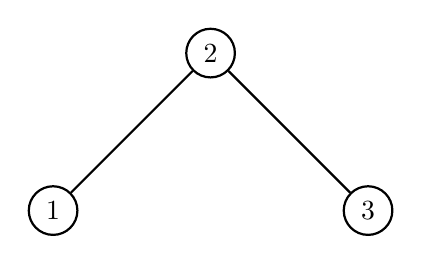
\begin{tikzpicture}[main node/.style={circle,thick,draw}]
  
  \node[main node] (n0) at (0,0) {1};
  \node[main node] (n1) at (2,2) {2};
  \node[main node] (n2) at (4,0) {3};
  \path[]
   (n0) [-, thick] edge node [] {} (n1)
   (n1) [-, thick] edge node [] {} (n2);
\end{tikzpicture}
\end{center}
\end{block}
\end{frame}

\begin{frame}
\frametitle{Graph Theory}
\begin{block}{Degree}
We define the \textbf{degree} of a vertex to be the number of \textbf{neighbors}, or vertices which are connected by an edge, the vertex has. This is generally denoted by $\text{deg}(x)$.
\end{block} 

\begin{block}{Regular}
A graph is said to be \textbf{$n$-regular} if the degree of all the vertices is $n$.
\end{block}
\end{frame}

\begin{frame}
\frametitle{Graph Theory}
\begin{block}{Example}
\only<1>{
$V = \{1, 2, 3\}$, $E = \{(1,2), (2,3)\}$.
\begin{center}
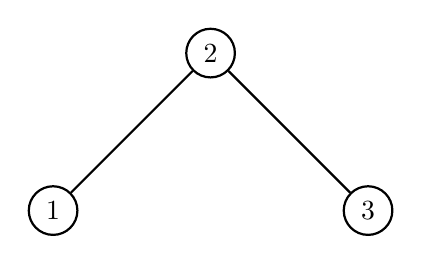
\begin{tikzpicture}[main node/.style={circle,thick,draw}]
  
  \node[main node] (n0) at (0,0) {1};
  \node[main node] (n1) at (2,2) {2};
  \node[main node] (n2) at (4,0) {3};
  \path[]
   (n0) [-, thick] edge node [] {} (n1)
   (n1) [-, thick] edge node [] {} (n2);
\end{tikzpicture}
\end{center}
We see $\text{deg}(2) = 2$, $\text{deg}(1) = 1$, and $\text{deg}(3) = 1$. This is therefore \textbf{not} regular.}
\only<2>{$V = \{1, 2, 3\}$, $E = \{(1,2), (1,3), (2,3)\}$.
\begin{center}
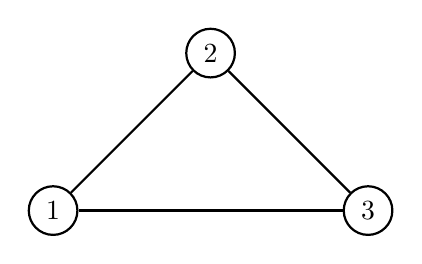
\begin{tikzpicture}[main node/.style={circle,thick,draw}]
  
  \node[main node] (n0) at (0,0) {1};
  \node[main node] (n1) at (2,2) {2};
  \node[main node] (n2) at (4,0) {3};
  \path[]
   (n0) [-, thick] edge node [] {} (n1)
   (n0) [-, thick] edge node [] {} (n2)
   (n1) [-, thick] edge node [] {} (n2);
\end{tikzpicture}
\end{center}
We see $\text{deg}(2) = 2$, $\text{deg}(1) = 2$, and $\text{deg}(3) = 2$. This is therefore \textbf{2-regular}.}
\end{block}
\end{frame}

\section{Markov Chains}

\begin{frame}
\frametitle{Markov Chains}
\begin{block}{Markov Property and Markov Chain}
A \textbf{Markov Chain} is a series of random variables $(X_0, X_1, \ldots)$ on a common state space $\Omega$ satisfying the \textbf{Markov Property}:
\[\mathbf{P} \{X_n = x_n \ | \ X_1 = x_1, \ldots, X_{n-1} = x_{n-1} \} = \mathbf{P} \{X_n = x_n \ | \ X_{n-1} = x_{n-1}\}. \]
\end{block} 
\begin{block}{Transition Matrix}
We can model Markov Chains using a \textbf{transition matrix}, which is a matrix with entries
\[ P(x,y) = \mathbf{P}\{X_n = y \ | \ X_{n-1} = x\} \]
\end{block}
\end{frame}

\begin{frame}
\frametitle{Markov Chains}
\begin{block}{Example}
\only<1>{
\begin{center}
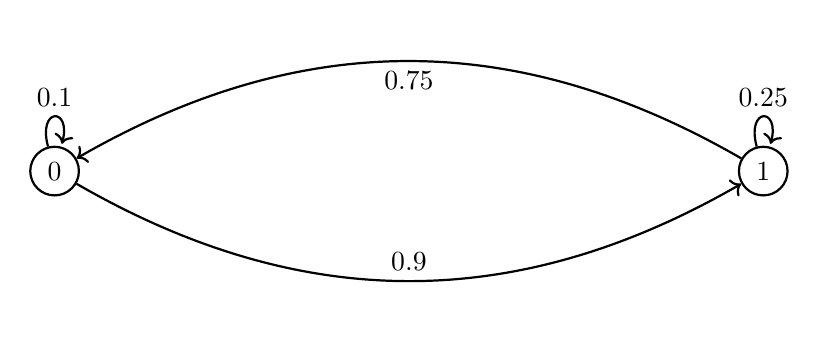
\begin{tikzpicture}[main node/.style={circle,thick,draw}]
  
  \node[main node] (n0) at (1,0) {0};
  \node[main node] (n1) at (10,0) {1};
  \path[]
   (n0) edge [loop above, thick] node {$0.1$} (n0)
   (n1) edge [loop above, thick] node {$0.25$} (n1)
   (n1) [->, bend right, thick] edge node [below] {$0.75$} (n0)
   (n0) [->, bend right, thick] edge node [above] {$0.9$} (n1);
\end{tikzpicture}
\end{center}}
\only<2>{
This Markov chain has transition matrix
\[P = \kbordermatrix{
& 0 & 1 \\
0 & 0.1 & 0.9 \\ 
1 & 0.75 & 0.25   \\
}
\]
}
\end{block}
\end{frame}

\begin{frame}
\frametitle{Markov Chains}
\begin{block}{Aperiodic and Irreducible}
We say our Markov Chain is \textbf{irreducible} if there exists a $t > 0$ for all $x,y \in \Omega$ such that 
\[ P^t(x,y) > 0. \]
We say that our Markov Chain is \textbf{aperiodic} if
\[ \gcd\{t \geq 1 \ | \ P^t(x,x) > 0\} = 1 \]
for all $x \in \Omega$.
\end{block}
\end{frame}

\begin{frame}
\frametitle{Markov Chains}
\begin{block}{Stationary Distribution}
If our Markov chain is \textbf{irreducible}, then we have that there exists a unique distribution $\pi$ such that 
\[ \pi P = \pi.\]
We call such a distribution a \textbf{stationary distribution}.
\end{block} 
\begin{block}{Limiting Distribution}
We call a distribution $\hat{\pi}$ a \textbf{limiting distribution} if 
\[\lim_{t \rightarrow \infty} P^t(x,y) = \hat{\pi}(y). \]
If our distribution is \textbf{aperiodic} and \textbf{irreducible}, then we have that the stationary distribution $\pi$ is the limiting distribution $\hat{\pi}$.
\end{block}
\end{frame}


\begin{frame}
\frametitle{Markov Chains}
\begin{block}{Example}
\only<1>{
\begin{center}
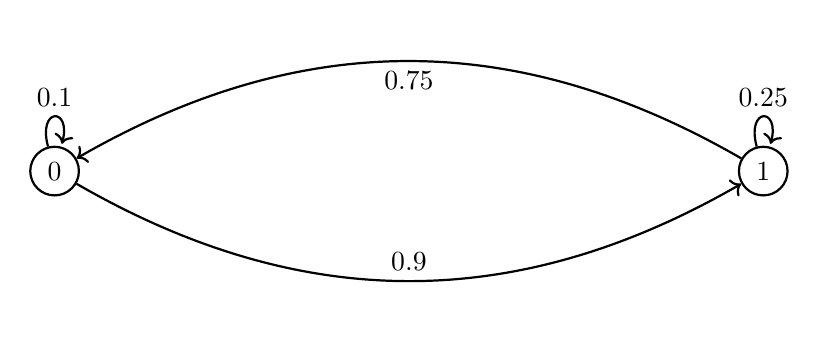
\begin{tikzpicture}[main node/.style={circle,thick,draw}]
  
  \node[main node] (n0) at (1,0) {0};
  \node[main node] (n1) at (10,0) {1};
  \path[]
   (n0) edge [loop above, thick] node {$0.1$} (n0)
   (n1) edge [loop above, thick] node {$0.25$} (n1)
   (n1) [->, bend right, thick] edge node [below] {$0.75$} (n0)
   (n0) [->, bend right, thick] edge node [above] {$0.9$} (n1);
\end{tikzpicture}
\end{center}}
\only<2>{
This Markov chain has transition matrix
\[P = \kbordermatrix{
& 0 & 1 \\
0 & 0.1 & 0.9 \\ 
1 & 0.75 & 0.25   \\
}
\]
Notice that this is \textbf{aperiodic} and \textbf{irreducible}, and so we have a stationary distribution. The stationary distribution is 
\[ \pi = \begin{bmatrix} \frac{5}{11} & \frac{6}{11} \end{bmatrix} \]
}
\end{block}
\end{frame}

\begin{frame}
\frametitle{Markov Chains}
\begin{block}{Simple Random Walk}
Given some graph $G$, we can define a \textbf{simple random walk on $G$} to be a Markov chain with state space $V$ and transition matrix
\[P(x,y) = \begin{cases} \frac{1}{\text{deg}(x)} \ \text{ if x and y are neighbors,} \\ 
0 \ \text{ otherwise.}\end{cases} \]
\end{block} \
\begin{block}{Lazy Random Walk}
Given some graph $G$, we can define a \textbf{lazy random walk on $G$} to be a Markov chain with state space $V$ and transition matrix
\[P(x,y) = \begin{cases} \frac{1}{2} \ \text{ if } x = y, \\ \frac{1}{2\text{deg}(x)} \ \text{ if x and y are neighbors,} \\ 0 \ \text{otherwise.} \end{cases} \]
\end{block}
\end{frame}

\section{Mixing Times}

\begin{frame}
\frametitle{Mixing Times}
\begin{block}{Total Variation Distance}
We define the \textbf{total variation distance} of two probability distributions $\mu$ and $\nu$ on a common state space $\Omega$ to be 
\[ ||\mu - \nu||_{TV} = \max_{A \subseteq \Omega} |\mu(A) - \nu(A)|. \]
In particular, we care about
\[ d(t) := ||P^t(x, \cdot) - \pi(\cdot)||_{TV}\]
\end{block} \
\begin{block}{Mixing Time}
We define the \textbf{mixing time} of a Markov chain to be 
\[t_{\text{mix}}(\epsilon) := \min \{t \ | \ d(t) \leq \epsilon \}. \]
\end{block}
\end{frame}

\begin{frame}
\frametitle{Motivation}
\begin{block}{Motivating Question}
Preforming a \textcolor{red}{random walk} on some \textcolor{red}{graph}, \textcolor{red}{how long does it take} until you are "\textcolor{red}{sufficiently random}?"
\end{block} 

\begin{block}{Theorem (Diaconis, Bayer '92)}
If you riffle shuffle a deck of size $n$, it takes approximately $ \frac{3}{2} \log_2(n)$ shuffles until the deck is "sufficiently random."
\end{block}

\end{frame}

\section{Coupling}

\begin{comment}
\begin{frame}
\frametitle{Coupling}
\begin{block}{Coupling of Probability Distributions}
We define the \textbf{coupling of two probability distributions} $\mu$ and $\nu$ over a common space $\Omega$ to be a pair of random variables $(X,Y)$ such that 
\[ \sum_{y \in \Omega} \mathbf{P}\{X = x, Y =y\} = \mathbf{P}\{X = x\} = \mu(x)\]
and
\[ \sum_{x \in \Omega} \mathbf{P}\{X = x, Y =y\} = \mathbf{P}\{Y = y\} = \nu(y).\]
\end{block}
\end{frame}
\end{comment}

\begin{frame}
\frametitle{Coupling}
\begin{block}{Coupling of Markov Chains}
We define a \textbf{coupling of two Markov chains} $(X_t)$ and $(Y_t)$ with transition matrix $P$ and common state space $\Omega$ to be a process $(X_t, Y_t)_{t=0}^{\infty}$ over the state space $\Omega \times \Omega$. Note that the two chains may (and in general we will want them to) have different starting distributions.
\end{block}
\end{frame}

\begin{frame}
\frametitle{Coupling}
\begin{block}{Markovian Coupling of Markov Chains}
We define a \textbf{Markovian coupling of two Markov chains} $(X_t)$ and $(Y_t)$ with common state space $\Omega$ and transition matrix $P$ to be the process $(X_t, Y_t)_{t=0}^{\infty}$ over $\Omega \times \Omega$, with the addendum that 
\[ \mathbf{P} \{X_{t+1} = x' \ | \ X_t = x, Y_t = y\} = P(x,x') \]
and
\[ \mathbf{P} \{Y_{t+1} = y' \ | \ X_t = x, Y_t = y \} = P(y,y'). \]
We will also require that $X_s = Y_s$ for some $s$ implies $X_t = Y_t$ for all $t \geq s$. A coupling is not a required to be Markovian (and it may not even be the optimal coupling), but in general we want our Markov chains to be Markovian.   
\end{block}
\end{frame}

\begin{comment}
\begin{frame}
\frametitle{Coupling}
\begin{block}{Example}
The \textbf{$n$-dimensional hypercube} is defined to be the set of binary strings of length $n$, $\{0,1\}^n$, such that two strings are connected by an edge if they differ in a component.
\begin{center}
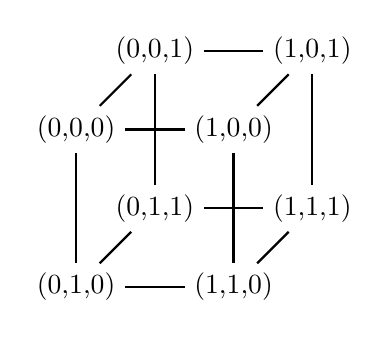
\begin{tikzpicture}
  
  \node (n0) at (4,4) {(1,0,0)};
  \node (n1) at (4,2) {(1,1,0)};
  \node (n2) at (2,2) {(0,1,0)};
  \node (n3) at (2,4) {(0,0,0)};

  \node (n4) at (3,5) {(0,0,1)};
  \node (n5) at (5,5) {(1,0,1)};
  \node (n6) at (3,3) {(0,1,1)};
  \node (n7) at (5,3) {(1,1,1)};

  \path[]
  (n0) [-, thick] edge node [] {} (n3);
  \path[] (n3) [-, thick] edge node [] {} (n2);
  \path[] (n3) [-, thick] edge node [] {} (n4);
\path[] (n2) [-, thick] edge node [] {} (n1);
\path[] (n2) [-, thick] edge node [] {} (n6);
\path[] (n4) [-, thick] edge node [] {} (n6);
\path[] (n4) [-, thick] edge node [] {} (n5);
\path[] (n6) [-, thick] edge node [] {} (n7);
\path[] (n0) [-, thick] edge node [] {} (n1);
\path[] (n0) [-, thick] edge node [] {} (n5);
\path[] (n5) [-, thick] edge node [] {} (n7);
\path[] (n1) [-, thick] edge node [] {} (n7);
\end{tikzpicture}
\end{center}
\end{block}
\end{frame}

\begin{frame}
\frametitle{Coupling}
\begin{block}{Example (cont.)}
We can study the mixing time of the lazy random walk on this hypercube using coupling. Say we were studying the uniform

\[(0,\mathbf{1},0)\]
\[(1,\mathbf{0},0)\]
\end{block}
\end{frame}
\end{comment}

\begin{frame}
\frametitle{Coupling}
\only<1>{
\begin{block}{Theorem}
Let 
\[ \tau := \min \{t \ | \ X_s = Y_s \text { for all } s \geq t \}.\]
Then we have 
\[d(t) \leq \max_{x,y \in \Omega} ||P^t(x, \cdot) - P^t(y, \cdot)||_{TV} \]
\[\leq \max_{x,y \in \Omega} \mathbf{P} \{\tau > t \ | \ X_0 = x, Y_0 = y\}  \]
\[ \leq \max_{x, y \in \Omega} \textcolor{black}{\frac{\mathbf{E}(\tau \ | \ X_0 = x, Y_0 = y)}{t}}\]
\end{block}
}
\only<2>{
\begin{block}{Theorem}
Let 
\[ \tau := \min \{t \ | \ X_s = Y_s \text { for all } s \geq t \}.\]
Then we have 
\[\textcolor{red}{d(t)} \leq \textcolor{red}{\max_{x,y \in \Omega} ||P^t(x, \cdot) - P^t(y, \cdot)||_{TV}} \]
\[\leq \max_{x,y \in \Omega} \mathbf{P} \{\tau > t \ | \ X_0 = x, Y_0 = y\}  \]
\[ \leq \max_{x, y \in \Omega} \textcolor{black}{\frac{\mathbf{E}(\tau \ | \ X_0 = x, Y_0 = y)}{t}}\]
\end{block}
}
\only<3>{
\begin{block}{Theorem}
Let 
\[ \tau := \min \{t \ | \ X_s = Y_s \text { for all } s \geq t \}.\]
Then we have 
\[\textcolor{red}{d(t)} \leq \max_{x,y \in \Omega} ||P^t(x, \cdot) - P^t(y, \cdot)||_{TV} \]
\[\leq \max_{x,y \in \Omega} \mathbf{P} \{\tau > t \ | \ X_0 = x, Y_0 = y\}  \]
\[ \leq \textcolor{red}{\max_{x, y \in \Omega} \frac{\mathbf{E}(\tau \ | \ X_0 = x, Y_0 = y)}{t}}\]
\end{block}
}
\end{frame}

\begin{frame}
\frametitle{Coupling}
\begin{block}{Example}
\begin{center}
\begin{tikzpicture}

\def \n {5}
\def \radius {3cm}
\def \margin {8} % margin in angles, depends on the radius

  \only<1,5>{\node[draw, circle,thick] at ({360/5 * (0)}:\radius) {0};}
  \only<2>{\node[draw, circle,thick,red] at ({360/5 * (0)}:\radius) {0};}
  \only<3-4>{\node[draw, circle,thick,blue ] at ({360/5 * (0)}:\radius) {0};}
  \draw[-, thick,>=latex] ({360/5 * (0)+\margin}:\radius) 
    arc ({360/5 * (0)+\margin}:{360/5 * (1)-\margin}:\radius);
   

  \node[draw, circle,thick] at ({360/5 * (1)}:\radius) {1};
  \draw[-, thick,>=latex] ({360/5 * (1)+\margin}:\radius) 
    arc ({360/5 * (1)+\margin}:{360/5 * (2)-\margin}:\radius);

  \node[draw, circle,thick] at ({360/5 * (2)}:\radius) {2};
  \draw[-, thick,>=latex] ({360/5 * (2)+\margin}:\radius) 
    arc ({360/5 * (2)+\margin}:{360/5 * (3)-\margin}:\radius);

  \only<1>{\node[draw, circle,thick] at ({360/5 * (3)}:\radius) {3};}
  \only<2-5>{\node[draw, circle,thick,red] at ({360/5 * (3)}:\radius) {3};}
  \draw[-, thick,>=latex] ({360/5 * (3)+\margin}:\radius) 
    arc ({360/5 * (3)+\margin}:{360/5 * (4)-\margin}:\radius);

  \only<1-4>{\node[draw, circle,thick] at ({360/5 * (4)}:\radius) {4};}
  \only<5>{\node[draw,red, circle,thick] at ({360/5 * (4)}:\radius) {4};}
  \only<1-3,5>{\draw[-, thick,>=latex] ({360/5 * (5 - 1)+\margin}:\radius) 
    arc ({360/5 * (5 - 1)+\margin}:{360/5 * (5)-\margin}:\radius);}
  \only<4>{\draw[-, blue,thick,>=latex] ({360/5 * (5 - 1)+\margin}:\radius) 
    arc ({360/5 * (5 - 1)+\margin}:{360/5 * (5)-\margin}:\radius);}


\end{tikzpicture}
\end{center}
\end{block}
\end{frame}


\begin{frame}
\frametitle{Coupling}
\begin{block}{Example}
If we measure the \textbf{clockwise distance} between the two walkers, this coupling gives us a new Markov chain on $\{0,1,\ldots, n\}$ to study.
\begin{center}
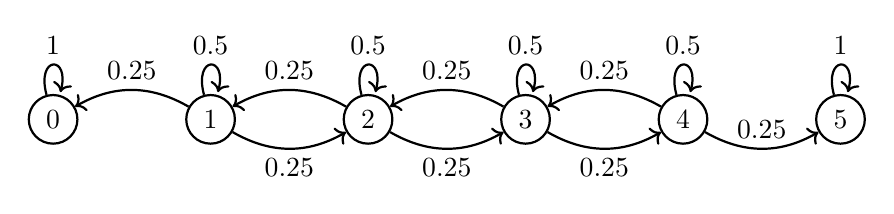
\begin{tikzpicture}[main node/.style={circle,thick,draw}]
  
  \node[main node] (n0) at (1,0) {0};
  \node[main node] (n1) at (3,0) {1};
  
  \node[main node] (n2) at (5,0) {2};
  \node[main node] (n3) at (7,0) {3};

  \node[main node] (n4) at (9,0) {4};
  \node[main node] (n5) at (11,0) {5};

  \path[]
   (n0) edge [loop above, thick] node {$1$} (n0)
   (n1) edge [loop above, thick] node {$0.5$} (n1)
   (n2) edge [loop above, thick] node {$0.5$} (n2)
   (n3) edge [loop above, thick] node {$0.5$} (n3)
   (n4) edge [loop above, thick] node {$0.5$} (n4)
   (n5) edge [loop above, thick] node {$1$} (n5)
   
   (n1) [->, bend right, thick] edge node [above] {$0.25$} (n0)
   (n2) [->, bend right, thick] edge node [above] {$0.25$} (n1)
   (n1) [->, bend right, thick] edge node [below] {$0.25$} (n2)
   (n3) [->, bend right, thick] edge node [above] {$0.25$} (n2)
   (n2) [->, bend right, thick] edge node [below] {$0.25$} (n3)
   (n4) [->, bend right, thick] edge node [above] {$0.25$} (n3)
   (n3) [->, bend right, thick] edge node [below] {$0.25$} (n4)
   (n4) [->, bend right, thick] edge node [above] {$0.25$} (n5);
   
\end{tikzpicture}
\end{center}
This gives us
\[ d(t) \leq \frac{n^2}{4t} \rightarrow t_{\text{mix}}(\epsilon) \leq \frac{n^2}{4\epsilon} \]
\end{block}
\end{frame}

\section{3-Regular Graphs}

\begin{frame}
\frametitle{3-Regular Graphs}
\begin{block}{Prism and M\"{o}bius ladder graphs }
\begin{center}
\begin{tikzpicture}[main node/.style={circle, thick, draw}, side node/.style={circle,thick,red,draw}]
  
  \node[main node] (n0) at (2,2) {};
  \node[main node] (n1) at (2,3) {};
  \node[main node] (n2) at (3,4) {};
  \node[main node] (n3) at (4,3) {};
  \node[main node] (n4) at (4,2) {};
  \node[main node] (n5) at (1,1) {};
  \node[main node] (n6) at (1,3) {};
  \node[main node] (n7) at (3,5) {};
 \node[main node] (n8) at (5,3) {};
 \node[main node] (n9) at (5,1) {};
 \path[] (n0) [-,thick] edge node [] {} (n1);
 \path[] (n1) [-,thick] edge node [] {} (n2);
 \path[] (n2) [-,thick] edge node [] {} (n3);
 \path[] (n3) [-,thick] edge node [] {} (n4);
 \only<1>{\path[] (n0) [-,thick] edge node [] {} (n4);}
 \only<2>{\path[] (n0) [-,thick, red] edge node [] {} (n4);}
 \only<3> {\path[](n5) [-,thick,red] edge node [] {} (n4);}
 \path[] (n0) [-,thick] edge node [] {} (n5);
 \path[] (n5) [-,thick] edge node [] {} (n6);
 \path[] (n6) [-,thick] edge node [] {} (n7);
 \path[] (n7) [-,thick] edge node [] {} (n8);
 \path[] (n8) [-,thick] edge node [] {} (n9);
 \only<1> {\path[] (n9) [-,thick] edge node [] {} (n5);}
 \only<2> {\path[] (n9) [-,thick,red] edge node [] {} (n5);}
 \only<3> {\path[](n9) [-,thick,red] edge node [] {} (n0);}
 \path[] (n1) [-,thick] edge node [] {} (n6);
 \path[] (n2) [-,thick] edge node [] {} (n7);
 \path[] (n3) [-,thick] edge node [] {} (n8);
 \path[] (n4) [-,thick] edge node [] {} (n9);
\end{tikzpicture}

\end{center}
\end{block}
\end{frame}

\begin{frame}
\frametitle{3-Regular Graphs}
\begin{block}{GP(n,k)}
Below is an example of $\text{GP}(6,2)$.
\begin{center}
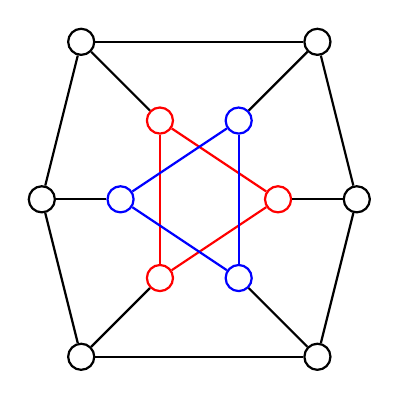
\begin{tikzpicture}[main node/.style={circle,thick,draw}, side node/.style={circle,thick,draw,red}, side side node/.style={circle, thick, draw, blue}]

\node[side node] (n0) at (2,3) {};
\node[side side node] (n1) at (3,3) {};
\node[side node] (n2) at (3.5,4) {};
\node[side side node] (n3) at (3,5) {};
\node[side node] (n4) at (2,5) {};
\node[side side node] (n5) at (1.5,4) {};
\node[main node] (n6) at (1,2) {};
\node[main node] (n7) at (4,2) {};
\node[main node] (n8) at (4.5,4) {};
\node[main node] (n9) at (4,6) {};
\node[main node] (n10) at (1,6) {};
\node[main node] (n11) at (0.5, 4) {};


\path[] (n6) [-, thick] edge node [] {} (n7);
\path[] (n7) [-, thick] edge node [] {} (n8);
\path[] (n8) [-, thick] edge node [] {} (n9);
\path[](n9) [-, thick] edge node [] {} (n10);
\path[](n10) [-, thick] edge node [] {} (n11);
\path[](n11) [-, thick] edge node [] {} (n6);

\path[](n0) [-, red, thick] edge node [] {} (n4);
\path[](n4) [-, red,thick] edge node [] {} (n2);
\path[](n2) [-, red, thick] edge node [] {} (n0);

\path[](n1) [-,blue,thick] edge node [] {} (n3);
\path[](n3) [-,blue,thick] edge node [] {} (n5);
\path[](n5) [-,blue,thick] edge node [] {} (n1);


\path[](n0) [-, thick] edge node [] {} (n6);
\path[](n1) [-,thick] edge node [] {} (n7);
\path[](n2) [-,thick] edge node [] {} (n8);
\path[](n3) [-,thick] edge node [] {} (n9);
\path[](n4) [-,thick] edge node [] {} (n10);
\path[](n5) [-,thick] edge node [] {} (n11);
\end{tikzpicture}
\end{center}
Notice that if we imagined a cycle on the inside, the nodes which are the same color would be distance \textbf{2} away from eachother.
\end{block}
\end{frame}


\begin{frame}
\frametitle{3-Regular Graphs}

\only<1>{
\begin{block}{Results}
Using coupling, we were able to determine that for M\"{o}bius ladder graphs and prism graphs of size $n$, the mixing time for a (slightly modified) lazy random walk is bounded by
\[ t_{\text{mix}}(\epsilon) \leq \frac{3n^2}{16\epsilon} + \frac{6}{\epsilon}, \]
and for the generalized Petersen graph $\text{GP}(n,k)$, the mixing time of the (slightly modified) lazy random walk is bounded by 
\[ t_{\text{mix}}(\epsilon) \leq \frac{3 |k|^2}{2\epsilon} + \frac{3}{2\epsilon} \bigg(\frac{n}{|k|}\bigg)^2 + \frac{15}{\epsilon},\]
where $|k| = n/\gcd(n,k)$.
\end{block}}
\only<2>{
\begin{block}{Results}
Using coupling, we were able to determine that for M\"{o}bius ladder graphs and prism graphs of size $n$, the mixing time for a (slightly modified) lazy random walk is bounded by
\[ t_{\text{mix}}(\epsilon) \leq \textcolor{red}{\frac{3n^2}{16\epsilon} } + \frac{6}{\epsilon}, \]
and for the generalized Petersen graph $\text{GP}(n,k)$, the mixing time of the (slightly modified) lazy random walk is bounded by 
\[ t_{\text{mix}}(\epsilon) \leq \textcolor{red}{\frac{3 |k|^2}{2\epsilon}} + \frac{3}{2\epsilon} \bigg(\frac{n}{|k|}\bigg)^2 + \frac{15}{\epsilon},\]
where $|k| = n/\gcd(n,k)$.
\end{block}
}
\end{frame}

\begin{frame}
\frametitle{3-Regular Graphs}
\begin{block}{Sketch of Proof (Prism Graph)}
\only<1>{
Couple based on inner cycle versus outer cycle.
\begin{center}
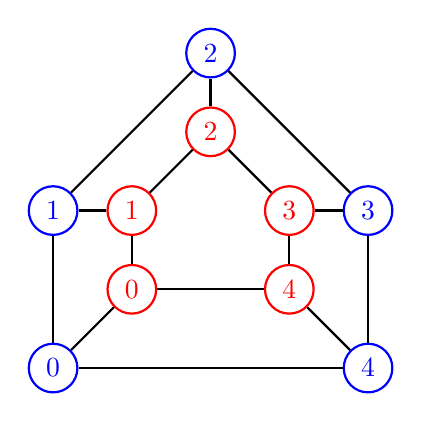
\begin{tikzpicture}[first node/.style={circle, red, thick, draw}, second node/.style={circle, blue, thick, draw}]
  
  \node[first node] (n0) at (2,2) {0};
  \node[first node] (n1) at (2,3) {1};
  \node[first node] (n2) at (3,4) {2};
  \node[first node] (n3) at (4,3) {3};
  \node[first node] (n4) at (4,2) {4};
  \node[second node] (n5) at (1,1) {0};
  \node[second node] (n6) at (1,3) {1};
  \node[second node] (n7) at (3,5) {2};
 \node[second node] (n8) at (5,3) {3};
 \node[second node] (n9) at (5,1) {4};
 \path[]
 (n0) [-,thick] edge node [] {} (n1)
 (n1) [-] edge node [] {} (n2)
 (n2) [-] edge node [] {} (n3)
 (n3) [-] edge node [] {} (n4)
 (n0) [-] edge node [] {} (n4)
 (n0) [-] edge node [] {} (n5)
 (n5) [-] edge node [] {} (n6)
 (n6) [-] edge node [] {} (n7)
 (n7) [-] edge node [] {} (n8)
 (n8) [-] edge node [] {} (n9)
 (n9) [-] edge node [] {} (n5)
 (n1) [-] edge node [] {} (n6)
 (n2) [-] edge node [] {} (n7)
 (n3) [-] edge node [] {} (n8)
 (n4) [-] edge node [] {} (n9);
\end{tikzpicture}
\end{center}}
\only<2>{
%Once coupled, we now shift our coupling so that our walkers move 'in' or 'out' together, and 'left' or 'right' independently of each other. Then this shifts the problem to the cycle, with the probability of staying in place being increased.
The coupling now shifts the problem to the random walk on the cycle, with increased probability of staying in place.
\begin{center}

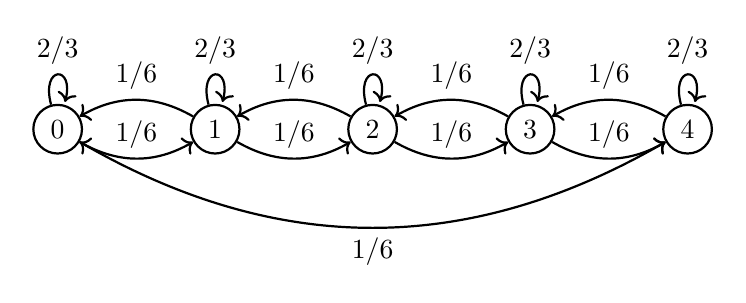
\begin{tikzpicture}[first node/.style={circle, thick, draw}]
  
  \node[first node] (n0) at (0,0) {0};
  \node[first node] (n1) at (2,0) {1};
  \node[first node] (n2) at (4,0) {2};
  \node[first node] (n3) at (6,0) {3};
  \node[first node] (n4) at (8,0) {4};
 \path[] (n0) edge [loop above, thick] node {$2/3$} (n0);
 \path[]  (n1) edge [loop above, thick] node {$2/3$} (n1);
 \path[]  (n2) edge [loop above, thick] node {$2/3$} (n2);
 \path[]  (n3) edge [loop above, thick] node {$2/3$} (n3);
 \path[]  (n4) edge [loop above, thick] node {$2/3$} (n4);
 \path[] (n0) [->, bend right, thick] edge node [above] {$1/6$} (n1);

 \path[] (n1) [->, bend right, thick] edge node [above] {$1/6$} (n2);

 \path[] (n2) [->, bend right, thick] edge node [above] {$1/6$} (n3);

 \path[] (n3) [->, bend right, thick] edge node [above] {$1/6$} (n4);

 \path[] (n4) [<->, bend left, thick] edge node [below] {$1/6$} (n0);

 \path[] (n4) [->, bend right, thick] edge node [above] {$1/6$} (n3);

 \path[] (n3) [->, bend right, thick] edge node [above] {$1/6$} (n2);

 \path[] (n2) [->, bend right, thick] edge node [above] {$1/6$} (n1);

 \path[] (n1) [->, bend right, thick] edge node [above] {$1/6$} (n0);

\end{tikzpicture}
\end{center}
}
\end{block}
\end{frame}

\begin{frame}
\frametitle{3-Regular Graphs}
\begin{block}{Sketch of Proof (M\"{o}bius Ladder Graph)}
\only<1>{
\begin{center}
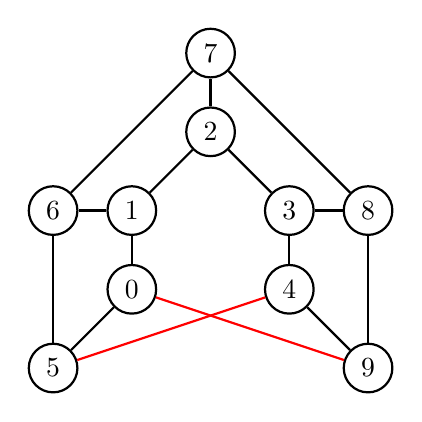
\begin{tikzpicture}[main node/.style={circle,thick, draw}]
  
  \node[main node] (n0) at (2,2) {0};
  \node[main node] (n1) at (2,3) {1};
  \node[main node] (n2) at (3,4) {2};
  \node[main node] (n3) at (4,3) {3};
  \node[main node] (n4) at (4,2) {4};
  \node[main node] (n5) at (1,1) {5};
  \node[main node] (n6) at (1,3) {6};
  \node[main node] (n7) at (3,5) {7};
 \node[main node] (n8) at (5,3) {8};
 \node[main node] (n9) at (5,1) {9};
 \path[] (n0) [-,thick] edge node [] {} (n1);
 \path[] (n1) [-,thick] edge node [] {} (n2);
 \path[] (n2) [-,thick] edge node [] {} (n3);
 \path[] (n3) [-,thick] edge node [] {} (n4);
 \path[] (n0) [-,thick] edge node [] {} (n5);
 \path[](n5) [-,thick,red] edge node [] {} (n4);
 \path[](n5) [-,thick] edge node [] {} (n6);
 \path[](n6) [-,thick] edge node [] {} (n7);
 \path[](n7) [-,thick] edge node [] {} (n8);
 \path[](n8) [-,thick] edge node [] {} (n9);
 \path[](n9) [-,thick,red] edge node [] {} (n0);
 \path[](n1) [-,thick] edge node [] {} (n6);
 \path[](n2) [-,thick] edge node [] {} (n7);
 \path[](n3) [-,thick] edge node [] {} (n8);
 \path[](n4) [-,thick] edge node [] {} (n9);
\end{tikzpicture}
\end{center}
}

\only<2>{
\begin{center}
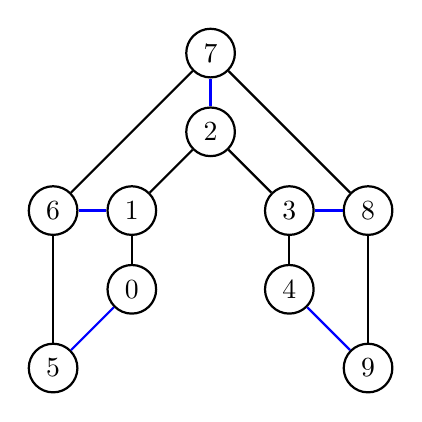
\begin{tikzpicture}[main node/.style={circle,thick, draw}]
  
  \node[main node] (n0) at (2,2) {0};
  \node[main node] (n1) at (2,3) {1};
  \node[main node] (n2) at (3,4) {2};
  \node[main node] (n3) at (4,3) {3};
  \node[main node] (n4) at (4,2) {4};
  \node[main node] (n5) at (1,1) {5};
  \node[main node] (n6) at (1,3) {6};
  \node[main node] (n7) at (3,5) {7};
 \node[main node] (n8) at (5,3) {8};
 \node[main node] (n9) at (5,1) {9};
 \path[] (n0) [-,thick] edge node [] {} (n1);
 \path[] (n1) [-,thick] edge node [] {} (n2);
 \path[] (n2) [-,thick] edge node [] {} (n3);
 \path[] (n3) [-,thick] edge node [] {} (n4);
 \path[] (n0) [-,thick,blue] edge node [] {} (n5);
 \path[](n5) [-,thick] edge node [] {} (n6);
 \path[](n6) [-,thick] edge node [] {} (n7);
 \path[](n7) [-,thick] edge node [] {} (n8);
 \path[](n8) [-,thick] edge node [] {} (n9);
 \path[](n1) [-,thick,blue] edge node [] {} (n6);
 \path[](n2) [-,thick,blue] edge node [] {} (n7);
 \path[](n3) [-,thick,blue] edge node [] {} (n8);
 \path[](n4) [-,thick,blue] edge node [] {} (n9);
\end{tikzpicture}
\end{center}
}

\only<3>{
\begin{center}
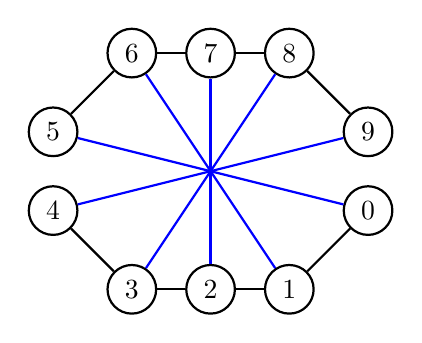
\begin{tikzpicture}[first node/.style={circle,thick,draw}, second node/.style={circle,thick,draw}]
  
  \node[first node] (n0) at (3,2) {3};
  \node[first node] (n1) at (4,2) {2};
  \node[first node] (n2) at (5,2) {1};
  \node[first node] (n3) at (6,3) {0};
  \node[first node] (n4) at (6,4) {9};
  \node[second node] (n5) at (5,5) {8};
  \node[second node] (n6) at (4,5) {7};
  \node[second node] (n7) at (3,5) {6};
  \node[second node] (n8) at (2,4) {5};
  \node[second node] (n9) at (2,3) {4};
 \path[] (n0) [-,thick,blue] edge node [] {} (n5);
 \path[] (n1) [-,thick,blue] edge node [] {} (n6);
 \path[](n2) [-,thick,blue] edge node [] {} (n7);
 \path[](n3) [-,thick,blue] edge node [] {} (n8);
 \path[](n4) [-,thick,blue] edge node [] {} (n9);

 \path[](n0) [-,thick] edge node [] {} (n1);
 \path[](n1) [-,thick] edge node [] {} (n2);
 \path[](n2) [-,thick] edge node [] {} (n3);
 \path[](n4) [-,thick] edge node [] {} (n5);
 \path[](n5) [-,thick] edge node [] {} (n6);
 \path[](n6) [-,thick] edge node [] {} (n7);
 \path[](n7) [-,thick] edge node [] {} (n8);

 \path[](n9) [-,thick] edge node [] {} (n0);
\end{tikzpicture}
\end{center}
}

\only<4>{
\begin{center}
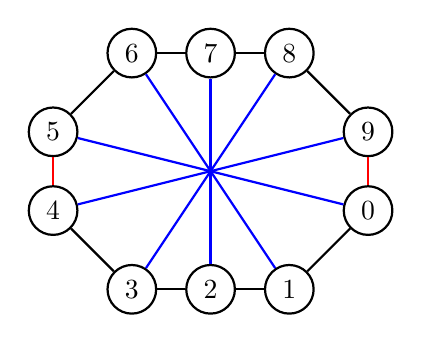
\begin{tikzpicture}[first node/.style={circle,thick,draw}, second node/.style={circle,thick,draw}]
  
  \node[first node] (n0) at (3,2) {3};
  \node[second node] (n1) at (4,2) {2};
  \node[second node] (n2) at (5,2) {1};
  \node[second node] (n3) at (6,3) {0};
  \node[first node] (n4) at (6,4) {9};
  \node[second node] (n5) at (5,5) {8};
  \node[second node] (n6) at (4,5) {7};
  \node[second node] (n7) at (3,5) {6};
  \node[second node] (n8) at (2,4) {5};
  \node[second node] (n9) at (2,3) {4};
 \path[] (n0) [-,thick,blue] edge node [] {} (n5);
 \path[] (n1) [-,thick,blue] edge node [] {} (n6);
 \path[](n2) [-,thick,blue] edge node [] {} (n7);
 \path[](n3) [-,thick,blue] edge node [] {} (n8);
 \path[](n4) [-,thick,blue] edge node [] {} (n9);
 \path[](n0) [-,thick] edge node [] {} (n1);
 \path[](n1) [-,thick] edge node [] {} (n2);
 \path[](n2) [-,thick] edge node [] {} (n3);
 \path[](n3) [-,thick,red] edge node [] {} (n4);
 \path[](n4) [-,thick] edge node [] {} (n5);
 \path[](n5) [-,thick] edge node [] {} (n6);
 \path[](n6) [-,thick] edge node [] {} (n7);
 \path[](n7) [-,thick] edge node [] {} (n8);
 \path[](n8) [-,thick,red] edge node [] {} (n9);
 \path[](n9) [-,thick] edge node [] {} (n0);
\end{tikzpicture}
\end{center}
}

\only<5>{
\begin{center}
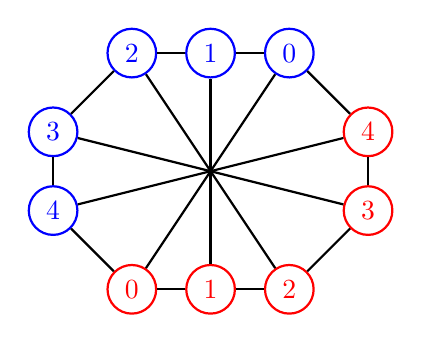
\begin{tikzpicture}[first node/.style={circle,thick,red,draw}, second node/.style={circle,thick,blue,draw}]
  
  \node[first node] (n0) at (3,2) {0};
  \node[first node] (n1) at (4,2) {1};
  \node[first node] (n2) at (5,2) {2};
  \node[first node] (n3) at (6,3) {3};
  \node[first node] (n4) at (6,4) {4};
  \node[second node] (n5) at (5,5) {0};
  \node[second node] (n6) at (4,5) {1};
  \node[second node] (n7) at (3,5) {2};
  \node[second node] (n8) at (2,4) {3};
  \node[second node] (n9) at (2,3) {4};
 \path[]
 (n0) [-,thick] edge node [] {} (n5)
 (n1) [-,thick] edge node [] {} (n6)
 (n2) [-,thick] edge node [] {} (n7)
 (n3) [-,thick] edge node [] {} (n8)
 (n4) [-,thick] edge node [] {} (n9)
 (n0) [-,thick] edge node [] {} (n1)
 (n1) [-,thick] edge node [] {} (n2)
 (n2) [-,thick] edge node [] {} (n3)
 (n3) [-,thick] edge node [] {} (n4)
 (n4) [-,thick] edge node [] {} (n5)
 (n5) [-,thick] edge node [] {} (n6)
 (n6) [-,thick] edge node [] {} (n7)
 (n7) [-,thick] edge node [] {} (n8)
 (n8) [-,thick] edge node [] {} (n9)
 (n9) [-,thick] edge node [] {} (n0);
\end{tikzpicture}
\end{center}

}

\only<6>{
Once on the same cycle, we can shift back to this Markov chain. We combine the results to find that the bound is the same as before.
\begin{center}

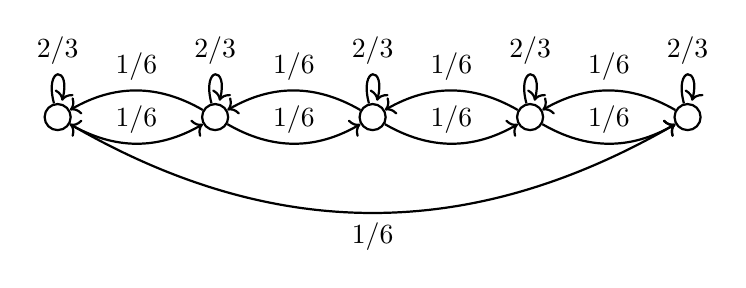
\begin{tikzpicture}[first node/.style={circle, thick, draw}]
  
  \node[first node] (n0) at (0,0) {};
  \node[first node] (n1) at (2,0) {};
  \node[first node] (n2) at (4,0) {};
  \node[first node] (n3) at (6,0) {};
  \node[first node] (n4) at (8,0) {};
 \path[] (n0) edge [loop above, thick] node {$2/3$} (n0);
 \path[]  (n1) edge [loop above, thick] node {$2/3$} (n1);
 \path[]  (n2) edge [loop above, thick] node {$2/3$} (n2);
 \path[]  (n3) edge [loop above, thick] node {$2/3$} (n3);
 \path[]  (n4) edge [loop above, thick] node {$2/3$} (n4);
 \path[] (n0) [->, bend right, thick] edge node [above] {$1/6$} (n1);

 \path[] (n1) [->, bend right, thick] edge node [above] {$1/6$} (n2);

 \path[] (n2) [->, bend right, thick] edge node [above] {$1/6$} (n3);

 \path[] (n3) [->, bend right, thick] edge node [above] {$1/6$} (n4);

 \path[] (n4) [<->, bend left, thick] edge node [below] {$1/6$} (n0);

 \path[] (n4) [->, bend right, thick] edge node [above] {$1/6$} (n3);

 \path[] (n3) [->, bend right, thick] edge node [above] {$1/6$} (n2);

 \path[] (n2) [->, bend right, thick] edge node [above] {$1/6$} (n1);

 \path[] (n1) [->, bend right, thick] edge node [above] {$1/6$} (n0);

\end{tikzpicture}
\end{center}
}
\end{block}
\end{frame}

\begin{frame}
\frametitle{3-Regular Graphs}
\begin{block}{"Triangulating"}
By "triangulating" a $3$-regular graph, we mean replace each vertex with a complete graph of size $3$.

\begin{center}
\begin{tikzpicture}[main node/.style={circle,thick,draw}]
  \only<1>{
  \node[main node] (n0) at (2,0) {};
  \node (n1) at (0,0) {};
  \node (n2) at (2,2) {};
  \node (n3) at (4,0) {};

  \path[] (n0) [-, thick] edge node [] {} (n1);
   \path[] (n0) [-, thick] edge node [] {} (n2);
   \path[] (n0) [-, thick] edge node [] {} (n3);
   }
   \only<2>{
 \node[main node] (n0) at (1,0) {};
  \node[main node] (n4) at (3,0) {};
  \node[main node] (n5) at (2,1) {};
  \node (n1) at (0,0) {};
  \node (n2) at (2,2) {};
  \node (n3) at (4,0) {};

  \path[] (n0) [-, thick] edge node [] {} (n1);
   \path[] (n2) [-, thick] edge node [] {} (n5);
   \path[] (n3) [-, thick] edge node [] {} (n4);
   \path[] (n0) [-, thick] edge node [] {} (n4);
 \path[] (n0) [-, thick] edge node [] {} (n5);
 \path[] (n4) [-, thick] edge node [] {} (n5);
}
\end{tikzpicture}
\end{center}
\end{block}
\end{frame}


\begin{frame}
\frametitle{3-Regular Graphs}
\only<1>{
\begin{block}{Example}
\begin{center}
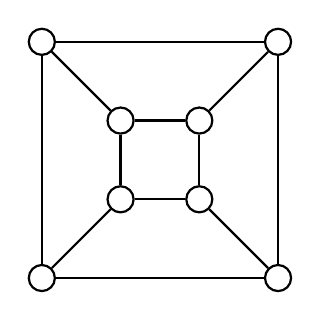
\begin{tikzpicture}[main node/.style={circle, thick, draw}, side node/.style={circle,thick,red,draw}]
  % inner cycle
  \node[main node] (n0) at (4,4) {};
  \node[main node] (n1) at (5,4) {};
  \node[main node] (n2) at (5,5) {};
  \node[main node] (n3) at (4,5) {};
  
  % outer cycle
  \node[main node] (n4) at (3,3) {};
  \node[main node] (n5) at (6,3) {};
  \node[main node] (n6) at (6,6) {};
  \node[main node] (n7) at (3,6) {};
\path[] (n0) [-, thick] edge node [] {} (n1)
(n1) [-, thick] edge node [] {} (n2)
(n2) [-] edge node [] {} (n3)
(n3) [-] edge node [] {}(n0)
(n4) [-] edge node [] {} (n5)
(n5) [-] edge node [] {} (n6)
(n6) [-] edge node [] {} (n7)
(n7) [-] edge node [] {} (n4)
(n0) [-] edge node [] {} (n4)
(n1) [-] edge node [] {} (n5)
(n2) [-] edge node [] {}(n6)
(n3) [-] edge node [] {}(n7);
\end{tikzpicture}
\end{center}
\end{block}
}
\only<2>{
\begin{block}{Example}
\begin{center}
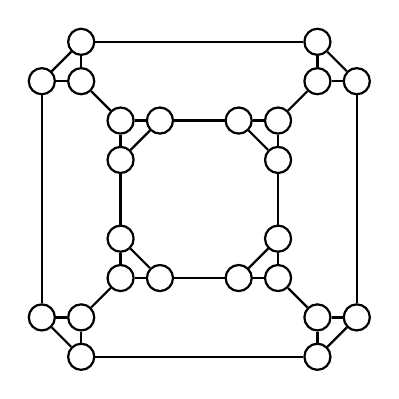
\begin{tikzpicture}[main node/.style={circle, thick, draw, minimum size=0.02cm}]
% inner
%triangle 1

% i/o
\node[main node] (n0) at (10, 10) {};

% u/d
\node[main node] (n1) at (10,10.5) {};

%l/r
\node[main node] (n2) at (10.5,10) {};

% triangle 2

%l/r
\node[main node] (n3) at (11.5,10) {};

%i/o
\node[main node] (n4) at (12,10) {};

%u/d
\node[main node] (n5) at (12, 10.5) {};

% triangle 3

%u/d
\node[main node] (n6) at (12, 11.5) {};

%i/o
\node[main node] (n7) at (12, 12) {};

%l/r
\node[main node] (n8) at (11.5, 12) {};

% triangle 4

%l/r
\node[main node] (n9) at (10.5, 12) {};

%i/o
\node[main node] (n10) at (10, 12) {};

%u/d
\node[main node] (n11) at (10, 11.5) {};

% outer
%triangle 5

% i/o
\node[main node] (n12) at (9.5,9.5) {};

%u/d
\node[main node] (n13) at (9, 9.5) {};

%l/r
\node[main node] (n14) at (9.5,9) {};

%triangle 6

%i/o
\node[main node] (n15) at (12.5, 9.5) {};

%u/d
\node[main node] (n16) at (13, 9.5) {};

%l/r
\node[main node] (n17) at (12.5, 9) {};

%triangle 7

%i/o
\node[main node] (n18) at (12.5, 12.5) {};

%u/d
\node[main node] (n19) at (13, 12.5) {};

%l/r
\node[main node] (n20) at (12.5, 13) {};

%triangle 8

% i/o
\node[main node] (n21) at (9.5, 12.5) {};

%l/r
\node[main node] (n22) at (9.5, 13) {};

%u/d
\node[main node] (n23) at (9, 12.5) {};

\path[] 
% inner cycle
% triangle 1
(n0) [-, thick] edge node [] {} (n1)
(n1) [-,thick] edge node [] {} (n2)
(n2) [-,thick] edge node [] {} (n0)

% triangle 1 -> triangle 2
(n2) [-,thick] edge node [] {} (n3)

% triangle 2
(n3) [-,thick] edge node [] {} (n4)
(n4) [-,thick] edge node [] {} (n5)
(n5) [-,thick] edge node [] {} (n3)

% triangle 2 -> triangle 3
(n5) [-,thick] edge node [] {} (n6)

% triangle 3
(n6) [-,thick] edge node [] {} (n7)
(n7)[-,thick] edge node [] {} (n8)
(n8)[-,thick] edge node [] {} (n6)

% triangle 3 -> triangle 4
(n8)[-,thick] edge node [] {} (n9)

% triangle 4
(n9)[-,thick] edge node [] {} (n10)
(n10)[-,thick] edge node [] {} (n11)
(n11)[-,thick] edge node [] {} (n9)

% triangle 4 -> triangle 1
(n11) [-, thick] edge node [] {} (n1)

% inner cycle -> outer cycle
(n0) [-,thick] edge node [] {} (n12)
(n4) [-,thick] edge node [] {} (n15)
(n7) [-,thick] edge node [] {} (n18)
(n10) [-,thick] edge node [] {} (n21)

% triangle 5
(n12) [-,thick] edge node [] {} (n13)
(n13) [-,thick] edge node [] {} (n14)
(n14) [-,thick] edge node [] {} (n12)

% triangle 6
(n15) [-,thick] edge node [] {} (n16)
(n16) [-,thick] edge node [] {} (n17)
(n17) [-,thick] edge node [] {} (n15)

% triangle 7
(n18) [-,thick] edge node [] {} (n19)
(n19) [-,thick] edge node [] {} (n20)
(n20) [-,thick] edge node [] {} (n18)

% triangle 8
(n21) [-,thick] edge node [] {} (n22)
(n22) [-,thick] edge node [] {} (n23)
(n23) [-,thick] edge node [] {} (n21)

% triangle 5 -> triangle 6
(n14) [-,thick] edge node [] {} (n17)

%triangle 6 -> triangle 7
(n16) [-,thick] edge node [] {} (n19)

% triangle 7 -> triangle 8
(n20) [-,thick] edge node [] {} (n22)

% triangle 8 -> triangle 5
(n23) [-, thick] edge node [] {} (n13)
;



\end{tikzpicture}
\end{center}
\end{block}
}
\end{frame}

\begin{frame}
\frametitle{3-Regular Graphs}
\begin{block}{Results}
\only<1>{
We found that when you triangulate the M\"{o}bius ladder graphs and prism graphs of size $n$, your mixing time transforms into
\[ t_{\text{mix}}(\epsilon) \leq \frac{15 n^2}{16 \epsilon} + \frac{87}{5 \epsilon}. \]
For the generalized Petersen graph $\text{GP}(n,k)$, it transforms into
\[ t_{\text{mix}}(\epsilon) \leq \frac{15 |k|^2}{2\epsilon} + \frac{15}{2\epsilon} \bigg(\frac{n}{|k|}\bigg)^2 + \frac{9}{\epsilon} \bigg(\frac{n}{|k|}\bigg) + \frac{9}{\epsilon} |k| + \frac{108}{\epsilon},\]
where $|k| = n/\gcd(n,k)$.
}

\only<2>{
We found that when you triangulate the M\"{o}bius ladder graphs and prism graphs of size $n$, your mixing time transforms into
\[ t_{\text{mix}}(\epsilon) \leq \textcolor{red}{\frac{15 n^2}{16 \epsilon}} + \frac{87}{5 \epsilon}. \]
For the generalized Petersen graph $\text{GP}(n,k)$, it transforms into
\[ t_{\text{mix}}(\epsilon) \leq \textcolor{red}{\frac{15 |k|^2}{2\epsilon}} + \frac{15}{2\epsilon} \bigg(\frac{n}{|k|}\bigg)^2 + \frac{9}{\epsilon} \bigg(\frac{n}{|k|}\bigg) + \frac{9}{\epsilon} |k| + \frac{108}{\epsilon},\]
where $|k| = n/\gcd(n,k)$.
}
\only<3>{
Using coupling, we were able to determine that for M\"{o}bius ladder graphs and prism graphs of size $n$, the mixing time for a (slightly modified) lazy random walk is bounded by
\[ t_{\text{mix}}(\epsilon) \leq \textcolor{red}{\frac{3n^2}{16\epsilon} } + \frac{6}{\epsilon}, \]
and for the generalized Petersen graph $\text{GP}(n,k)$, the mixing time of the (slightly modified) lazy random walk is bounded by 
\[ t_{\text{mix}}(\epsilon) \leq \textcolor{red}{\frac{3 |k|^2}{2\epsilon}} + \frac{3}{2\epsilon} \bigg(\frac{n}{|k|}\bigg)^2 + \frac{15}{\epsilon},\]
where $|k| = n/\gcd(n,k)$.
}
\end{block}
\end{frame}


\begin{comment}

\begin{frame}
\frametitle{3-Regular Graphs}
\begin{block}{Remaining Questions}
We see that for these nice classes of $3$-regular graphs, the mixing time of the triangulated graph is asymptotically at most $5$ times larger. Can we generalize this result to all vertex transitive $3$-regular graphs? Furthermore, can we extend it to all $3$-regular graphs? Are the bounds we found above tight, or can we improve them? Does a similar result apply to lower bounds on these mixing times?
\end{block}
\end{frame}

\end{comment}
\begin{frame}
\frametitle{3-Regular Graphs}
\begin{block}{Remaining Questions}
\begin{itemize}
\item Can we generalize this result to all vertex transitive $3$-regular graphs? 
\item Can we extend it to all $3$-regular graphs? 
\item Are the bounds we found above tight, or can we improve them? 
\item Does a similar result apply to lower bounds on these mixing times?
\end{itemize}
\end{block}
\end{frame}

\end{document}